
% This LaTeX was auto-generated from MATLAB code.
% To make changes, update the MATLAB code and republish this document.

\documentclass{article}
\usepackage{graphicx}
\usepackage{color}

\sloppy
\definecolor{lightgray}{gray}{0.5}
\setlength{\parindent}{0pt}

\begin{document}

    
    \begin{verbatim}
clc; close all; clear all;

Fs = 100; % Sampling frequency
t = 0:1/Fs:1; % Time vector of 1 second

x = 10*cos(10*t) + 20*cos(20*t); % Define signal

nfft = 8192; % Length of FFT

% SINGLE SIDED
f1 = (0:nfft/2-1)*Fs/nfft; % Define frequency vector
X1 = fft(x,nfft); % Take FFT of length nfft
X1 = X1(1:nfft/2);% FFT is symmetric, throw away second half

% DOUBLE SIDED
% Take fft of length nfft and shift it
f2 = (-nfft/2:nfft/2-1)*Fs/nfft; % Define frequency vector
X2 = fftshift(fft(x,nfft)); % Take FFT and shift

figure();
subplot(311);
plot(t,x); grid on;
xlabel('Time (sec)');
ylabel('Amplitude');
title('Signal x(t)');

subplot(312);
plot(f1,abs(X1)); grid on;
xlabel('Frequency (Hz)');
ylabel('Power');
title('Single-Sided Power Spectrum of x(t)');

subplot(313);
plot(f2,abs(X2)); grid on;
xlabel('Frequency (Hz)');
ylabel('Power');
title('Double-Sided Power Spectrum of x(t)');

figure();
plot(f2,abs(X2)); grid on;
xlabel('Frequency (Hz)');
ylabel('Power');
title('Double-Sided Power Spectrum of x(t)');
\end{verbatim}

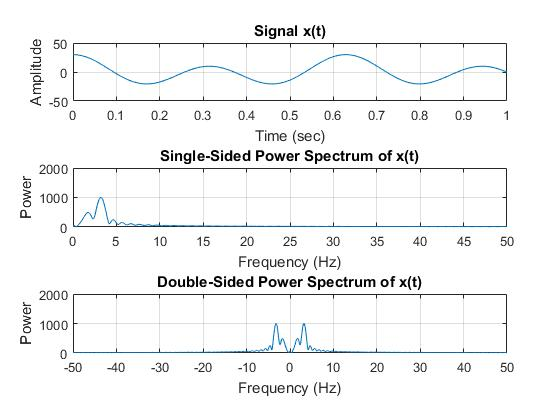
\includegraphics [width=4in]{ee5420_1_5_2_01.jpg}

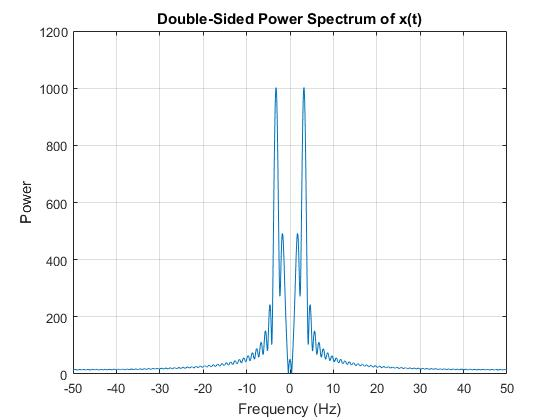
\includegraphics [width=4in]{ee5420_1_5_2_02.jpg}



\end{document}
    
